% importa variabili globali
% definizione variabili globali
\def\GRUPPO {\textit{DazzleWorks}}

\def\PROGETTO {\textbf{Premi}}

\def\COMMITTENTE {Prof. Vardanega Tullio, \\ & Dr. Cardin Riccardo}

\def\EMAIL {dazzleworksgroup@gmail.com}

\def\LOGO {../../template/img/logo.png}

\def\INTESTAZIONE {../../template/img/intestazione.png}
\def\PIEDIPAGINA {../../template/img/piedipagina.png}

\def\G {{\small $_G$}}



% definizione variabili locali
\def\DOCUMENTO{Specifica tecnica}
\def\VERSIONE{1.0.0}

\def\DESCRIZIONE{<Info documento}

\def\REDATTORE {<Redattore>}
\def\VERIFICATORE {<Verificatore>}
\def\RESPONSABILE {Carraro Nicola}

\def\USO {Esterno}

\def\DISTRIBUZIONE {\GRUPPO{}\\ & \COMMITTENTE{}\\}

\def\DESCRIZIONE {Specifica tecnica e architettura dell'applicazione Premi}


% abilita (true) / disabilita (false) indice, lista tabelle, lista figure
\def\INDICE	{true}
\def\TABELLE {true}
\def\FIGURE {true}


% importa struttura
\documentclass[a4paper]{article}

% ----- definizioni -----
\def\TITLE		{\mbox{\GRUPPO}}
\def\SUBTITLE	{\SIGLA, \PROGETTO}


% ----- nuovi comandi -----
% fornisce il caption per riferirsi ad una particolare sezione
\newcommand{\numref}[1]{\textsf{\textsl{``\nameref{#1}'' (\ref{#1})}}}


% ----- package -----
\usepackage[T1]{fontenc}   % codifica dei font in uscita
\usepackage[utf8x]{inputenc}   % lettere accentate da tastiera
\usepackage[italian]{babel}   % lingua principale del documento
\usepackage[a4paper, top= 3cm, bottom= 3cm, left= 3cm, right= 3cm, bindingoffset= 5mm]{geometry} % impostazione margini

\usepackage{amssymb} %

\usepackage{booktabs} % comandi aggiuntivi per le tabelle

\usepackage{calc} % espressioni aritmetiche
\usepackage{caption} % descrizione figure, ecc
\usepackage{chapterbib} % inclusione delle bibliografie

\usepackage{datatool} % manipolazione dati
\usepackage{dcolumn} % array in tabular

\usepackage{epstopdf} % conversione eps--> pdf
\usepackage{enumitem} % personalizzazione liste
\usepackage{eurosym} % simbolo euro

\usepackage{fancyhdr}   %personalizzazione dello stile
\usepackage{float} % definizione di oggetti floating (es. figure, tabelle)
\usepackage[bottom]{footmisc} % personalizzazione note

\usepackage[toc]{glossaries}	% glossario
\usepackage{graphicx, subfigure} % pacchetto grafica testo
\usepackage{grffile} % estende gestione filename graphic

\usepackage[colorlinks=true, urlcolor=blue, citecolor=black, linkcolor=black, hyperindex, breaklinks]{hyperref} % gestione dei link

\usepackage{ifthen}	% costrutto ifthenelse

% \usepackage{listings} % inserimento pezzi di codice
\usepackage{longtable} % tabelle su più pagine

\usepackage{pgf} % grafica postscript e PDF
\usepackage{pgfplots}	% composizione di grafici
\pgfplotsset{/pgf/number format/use comma, compat=newest}	% opzioni per i grafici

\usepackage{multirow} % span multiriga

\usepackage{tabularx, array} % crea paragrafi a colonne
\usepackage{titlesec} % personalizzazione titoli
\usepackage{tikz} % gestione delle formule
\usepackage{totpages} % conta numero pagine

\usepackage{soul} % gestione letterspacing
\usepackage{subfigure} % gestione delle sottofigure

\usepackage{verbatim} % inserimento testo verbatim, non interpretato

\usepackage{wallpaper} % gestione background

\usepackage{xspace} % spazi automatici per le macro


% ----- posizione etichette -----
\captionsetup{tableposition=top, figureposition=bottom, font=small}


% ----- glossario -----
\loadglsentries{../../glossario/glossario.tex}
\renewcommand*{\glssymbolsgroupname}{Simboli}


% ----- stile pagina -----
\pagestyle{fancy}

	% header
	\fancypagestyle {firststyle} {	% definizione stile "firststyle"
		\fancyhf{}
	}

	% indentazione paragrafo
	%\setlength{\parindent} {0pt}
	\setlength{\headheight} {25pt}

	% intestazione
	\lhead{}
	\rhead{\nouppercase{\leftmark}}
	\renewcommand{\headrulewidth}{0pt}  % no linea sotto intestazione

	% piè di pagina
	\lfoot{\footnotesize{{\DOCUMENTO} \\ {\VERSIONE}}}
	\cfoot{}
	\rfoot{\thepage}
	\renewcommand{\footrulewidth}{0pt}   % no linea sopra piè di pagina


% ----- inizio documento -----
% ----- prima pagina -----
\begin{document}
\thispagestyle{firststyle}

\begin{center}

%   \vspace{7cm}
	\textbf{{\fontsize{40pt}{41pt}\selectfont \PROGETTO}} \\
	\rule{8cm}{3pt}
   
   \vspace{4cm}
   \includegraphics[height= 4cm] {\LOGO}
   
	\vspace{1cm}
   {\fontsize{30pt}{31pt}\selectfont \textbf{\GRUPPO}}
	
	\vspace{5cm}
	{\fontsize{18pt}{24pt}\selectfont \textbf{\DOCUMENTO}}
	
%	\vspace{1cm}
	\begin{center}
		\begin{tabular}{r|l}
				\textbf{Versione} & \VERSIONE \\
				\textbf{Redattori} & \REDATTORE \\
				\textbf{Verificatori} & \VERIFICATORE \\
				\textbf{Responsabili} & \RESPONSABILE \\
				\textbf{Uso} & \USO \\
				\textbf{Lista di distribuzione} & \DISTRIBUZIONE
		\end{tabular}
	\end{center}

	\vspace{1cm}
	\textbf{\DESCRIZIONE}

\end{center}


\newpage

% ----- pagine successive -----
\ULCornerWallPaper{1}{\INTESTAZIONE}
\LLCornerWallPaper{1}{\PIEDIPAGINA}

%\thispagestyle{empty}

\newpage

% diario delle modifiche


% numerazione pagine indici
\pagenumbering{Roman}



% importa indici
% definizione indice
\ifthenelse{\equal{\INDICE}{true}}
	{\tableofcontents \newpage}{}

% definizione lista tabelle
%\ifthenelse{\equal{\TABELLE}{true}} 
%	{\listoftables \newpage}{}

% definizione lista figure
\ifthenelse{\equal{\FIGURE}{true}}
	{\listoffigures \newpage}{}


% numerazione pagine
\pagenumbering{arabic}

	% formato visualizzazione
	\rfoot{\thepage ~di~\pageref{TotPages}}


% separatore
\iffalse
	AOjvdYTJD7mcIIYItfsNiYPbmTTogRSP9hrrb2XPE1laMyQ9NHrPgTCTxnW0eV1YcM3Wqh7t5qThjczeXWq3O5FJ7BBQjoWZovC5
\fi


% importa parti documento

\section{Introduzione}
\subsection{Scopo del documento}
	Il documento ha lo scopo di definire l'architettura generale e i \gls{design pattern} da utilizzare secondo i quali verrà sviluppato il software del progetto Premi.

\subsection{Scopo del prodotto}
Lo scopo del progetto è realizzare un software per un sistema di rappresentazione di \gls{slide} sfruttando la tecnologia  \gls{HTML5}. Lo scopo principale è quello di creare un prodotto che sia di qualità comparabile, in prestazioni, funzionalità ed effetti visivi, ai maggiori concorrenti già presenti sul mercato (Prezi, Powerpoint, Keynote, Impress, ...).

\subsection{Glossario}
Per prevenire ed evitare qualsiasi dubbio e per permettere una maggiore chiarezza e comprensione del testo su termini ambigui, abbreviazioni e acronimi utilizzati nei vari documenti, essi sono stati raccolti nel \textit{Glossario v2.0.0} nel quale si possono trovare tutte le informazioni desiderate.
Al fine di rendere subito evidente un termine presente nel \textit{Glossario}, esso verrà marcato con il pedice \G\footnote{Per le istruzioni si rimanda al documento \textit{Norme di Progetto v2.0.0} .}.

\subsection{Riferimenti}

\subsubsection{Normativi}
	\begin{itemize}
		\item \textbf{Analisi dei Requisiti:} \textit{Analisi dei Requisiti v3.0.0};
		\item \textbf{Norme di Progetto:} \textit{Norme di Progetto v2.0.0}.
	\end{itemize}

\subsubsection{Informativi}
	\begin{itemize}
		\item \textbf{Design Patterns, elementi per il riuso di software ad oggetti:} Gamma, Helm, Johnson, Vlissides;
		\item \textbf{SWEBOK v3, Guide to the Software Engineering Body of Knowledge:} IEEE Computer Society;
		\item \textbf{Ingegneria del software} Ian Sommerville, Parte terza: \textit{progettazione};
		\item \textbf{Slide del corso:}
				\begin{itemize}
					\item \textbf{Diagrammi delle classi}: \url{http://www.math.unipd.it/~tullio/IS-1/2014/Dispense/E2a.pdf};
					\item \textbf{Diagrammi dei package}: \url{http://www.math.unipd.it/ ~tullio/IS-1/2014/Dispense/E2b.pdf};
					\item \textbf{Pattern}:
					\begin{itemize}
						\item \textit{Architetturali}
							\begin{itemize}
								\item \url{http://www.math.unipd.it/~tullio/IS-1/2014/Dispense/E9.pdf};
								\item \url{http://www.math.unipd.it/~rcardin/pdf/Design\%20Pattern\%20Architetturali\%20-\%20Model\%20View\%20Controller\_4x4.pdf};
							\end{itemize}
						\item \textit{Strutturali}:
						\begin{itemize}
						\item \url{http://www.math.unipd.it/~tullio/IS-1/2014/Dispense/E6.pdf};
						\end{itemize}
						\item \textit{Creazionali}:
						\begin{itemize}
						\item \url{http://www.math.unipd.it/~tullio/IS-1/2014/Dispense/E7.pdf};
						\end{itemize}
						\item \textit{Comportamentali}:
						\begin{itemize}
						\item \url{http://www.math.unipd.it/~tullio/IS-1/2014/Dispense/E8.pdf};
						\end{itemize}
					\end{itemize}
					\item \textbf{Documentazione di Chart.js}: \url{http://chartjs.org/docs};
					\item \textbf{Documentazione di Angular.js}: \url{https://docs.angularjs.org/guide};
					\item \textbf{Documentazione di Reveal.js}: \url{http://github.com/hakimel/reveal.js};
					\item \textbf{Documentazione di Fabric.js}: \url{http://fabricjs.com};
					\item \textbf{Manuale di MongoDb}: \url{https://docs.mongodb.org/manual};
					\item \textbf{Documentazione di Foundation}: \url{http://foundation.zurb.com/docs};
					\item \textbf{Documentazione di Php}: \url{http://php.net/docs.php}.
				\end{itemize}

	\end{itemize}


\newpage

\section{Tecnologie utilizzate}
In questa sezione verranno descritte le tecnologie che saranno usate nel progetto.


\subsubsection{AJAX}
È una tecnica di sviluppo software che permette di realizzare applicazioni web interattive tramite chiamate asincrone tra client e server.
La scelta di AJAX è dovuta alla necessità di scambiare dati con il server e di aggiornare porzioni di pagine web senza dover ricaricare l'intera pagina.

\subsubsection{HTML5}
È un linguaggio di markup per la strutturazione delle pagine web, pubblicato come W3C Recommendation da ottobre 2014.
I vantaggi offerti da questa tecnologia sono il supporto canvas per la creazione di figure e animazioni utilizzando il linguaggio JavaScript. Ciò permette di avere una superficie dove disegnare la nostra presentazione e di realizzare effetti grafici. Inoltre è ampiamente diffuso sia in ambiente \textit{desktop} sia in ambiente \textit{mobile}.

\subsubsection{PHP}
È un linguaggio di programmazione interpretato, il quale interprete è disponibile con licenza open-source.
L'uso di questa tecnologia è motivato dalla necessità di avere un linguaggio lato server che ci permette di interfacciarci con il database e di generare degli script di web-scraping da utilizzare per l'estrapolazione e l'elaborazione di dati ottenuti in real-time da sorgenti esterne in quanto, a causa della same-origin-policy, sarebbe impossibile ottenerli dal lato client. Inoltre, PHP è particolarmente adatto a rispondere alle chiamate in AJAX da parte del client.

\subsubsection{Angular.js}
È un framework che permette di realizzare applicazioni web con l'obiettivo di semplificare lo sviluppo e il test delle applicazioni favorendo un approccio dichiarativo allo sviluppo client-side. Basato sul pattern MVC, Angular funziona attraverso l'inclusione di tag e attributi addizionali che vengono interpretati come delle direttive.
Il vantaggio di utilizzare questo framework è quindi quello di semplificare lo sviluppo delle pagine web.

\subsubsection{Reveal.js}
È un framework che permette di creare delle presentazioni interattive in HTML.
L'utilizzo di Reveal.js è stato scelto per la sua strutturazione della presentazione che si adatta alla nostra visione del progetto, soprattutto per quanto riguarda il modo di effettuare la presentazione.

\subsubsection{Mustache}

\subsubsection{JQuery}
È una libreria di funzioni Javascript per le applicazioniweb, che si propone come obiettivo quello di semplificare la manipolazione, la gestione degli eventi e l'animazione delle pagine HTML. La sintassi di JQuery è studiata per semplificare la navigazione dei documenti, la selezione degli elementi DOM, creare animazioni, gestire eventi e implementare funzionalità AJAX.

\subsubsection{MongoDB}

\subsubsection{CSS3}

\subsubsection{Bootstrap}

\newpage

\section{Descrizione architettura}
\subsection{Metodo e formalismo di specifica}
L'architettura del progetto verrà esposta seguendo il metodo top-down, si partirà, cioè, dal livello più generale per poi scendere nel dettaglio. I diagrammi di classe, attività e sequenza saranno conformi al formalismo UML 2.x, come previsto nelle Norme di Progetto v1.0.0.

\subsection{Architettura generale}
L'architettura del prodotto che vogliamo realizzare segue il pattern three-tier, che prevede la suddivisione dell'applicazione in tre diversi strati. I tre strati sono dedicati rispettivamente all'interfaccia utente, alla logica funzionale e alla gestione dei dati persistenti e comunicano tra loro secondo le linee generali del modello client-server. L'architettura three-tier permette una maggiore scalabilità e manutenibilità dell'applicazione in quanto è possibile modificare o sostituire uno strato indipendentemente dagli altri. Attraverso la seguente presenteremo i tier dell'architettura adattati al nostro progetto, che saranno approfonditi nel dettaglio nelle sezioni successive del documento.

\begin{figure}[h]
	\centering
	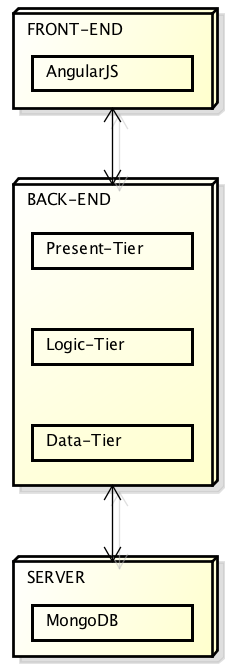
\includegraphics[height=0.6\textheight]{img/architettura_generale}
	\caption[Architettura generale del sistema]{Architettura generale del sistema}
\end{figure}

\textbf{Presentation-Tier}: contiene il front-end dell'applicazione, che si occupa della presentazione dei dati all'utente. Funge da interfaccia tra l'utente e il back-end, interagendo con il tier sottostante.

\textbf{Logic-Tier}: comunica con il livello superiore elaborando le richieste generate da esso e recuperando i dati dal livello inferiore. Questo strato è a sua volta organizzato con un'architettura three-tier per la gestione del back-end dell'applicazione.

\textbf{Data-tier}: questo livello è costituito dal database dell'applicazione ed è dove vengono memorizzate e recuperate le informazioni. Nel nostro caso il database è di tipo non relazionale.

\newpage

\section{Architettura Front-End}
\subsection{Premi::Front-End}
	\subsubsection*{Informazioni sul package}
		\begin{figure}[h]
			\centering
			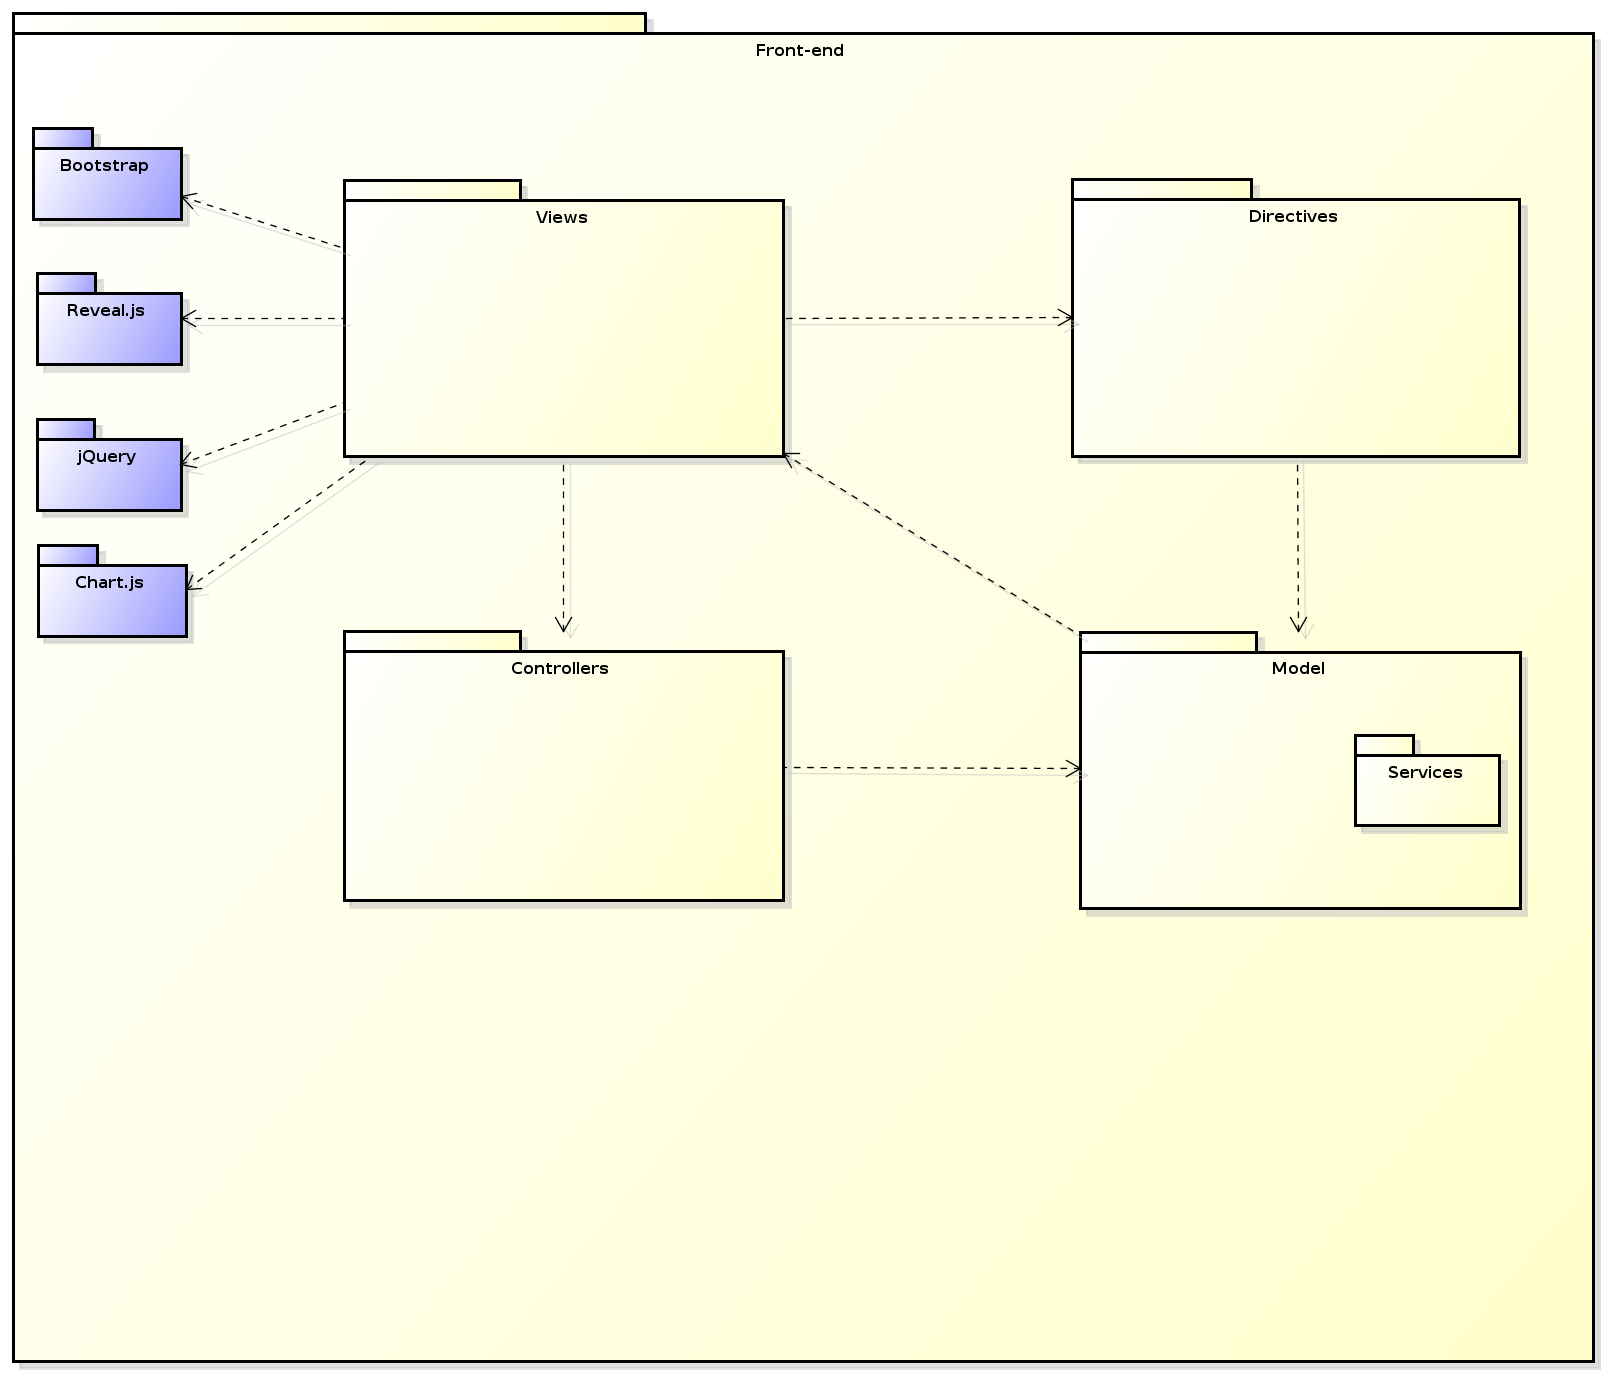
\includegraphics[width=0.7\linewidth]{img/front-end-package}
			\caption[Premi::Front-End]{Premi::Front-End}
		\end{figure}
		Il package contiene le varie componenti della parte di front-end dell'applicazione.

	\subsubsection*{Package contenuti:}
		\begin{itemize}
			\item \textbf{View:} Package contenente le views della componente front-end dell'applicazione;
			\item \textbf{Directives:} Package contenente le directives che compongono la view;
			\item \textbf{Model:} Package che definiscono la bussiness logic dell'applicazione;
			\item \textbf{Controller:} Package contenente i controller della parte front-end dell'applicazione.
		\end{itemize}


\subsection{Premi::Front-End::Model}
	\subsubsection*{Informazioni sul package}
		\begin{figure}[h]
			\centering
			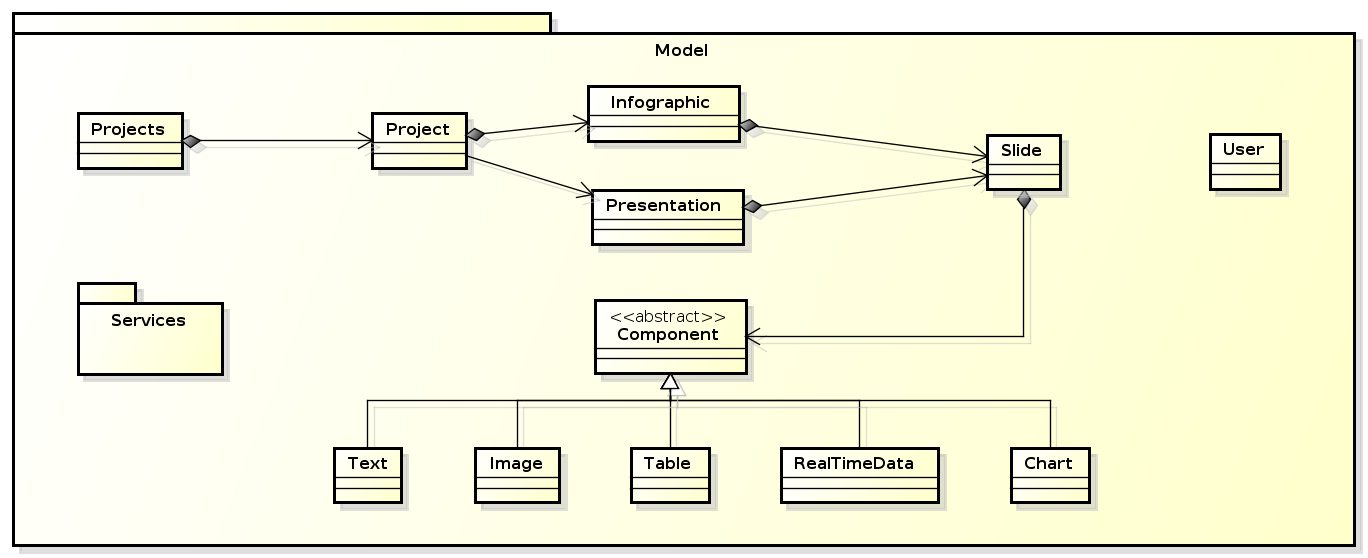
\includegraphics[width=0.7\linewidth]{img/front-end-package_model}
			\caption[Premi::Front-End::Model]{Premi::Front-End::Model}
		\end{figure}
		Il package serve per mantenere i dati relativi al \textit{front-end} e tutta la loro logica di business.

	\subsubsection*{Classi contenute:}
		\begin{itemize}
			
		 \item Premi::Front-End::Model::Projects:
			\begin{itemize}
				\item \textbf{Descrizione}:classe per la gestione di una collezione di progetti.Un progetto racchiude una presentazione e zero o più infografiche.
				\item \textbf{Relazioni con altre classi}:
				\begin{itemize}
					\item Premi::Front-End::Model::Project.
				\end{itemize}
			\end{itemize}
		
		\item Premi::Front-End::Model::Project: 
			 \begin{itemize}
				\item \textbf{Descrizione}: classe per la gestione di un progetto.
				\item \textbf{Relazioni con altre classi}:
				\begin{itemize}
					\item Premi::Front-End::Model::Presentation.
					\item Premi::Front-End::Model::Infographic.
				\end{itemize}
			\end{itemize}
		
		 \item Premi::Front-End::Model::Infographic:
			\begin{itemize}
				\item \textbf{Descrizione}: classe per la gestione di una infografica. Un'infografica ha il compito di raggruppare piu slide in un template grafico scelto dall'utente in un ordine impostabile di volta in volta.
				\item \textbf{Relazioni con altre classi}:
				\begin{itemize}
					\item Premi::Front-End::Model::Slide.
				\end{itemize}
			\end{itemize}
		 
		 \item Premi::Front-End::Model::Presentation:
			\begin{itemize}
				\item \textbf{Descrizione}: classe per la gestione di una presentazione. Una presentazione raggruppa più slide. Per la visualizzazione delle presentazioni è stato scelto di utilizzare il framework Reveal.js che permette di avere una visualizzazione a griglia, di conseguenza una presentazione deve memorizzare anche le coordinate delle sue slide.
				\item \textbf{Relazioni con altre classi}:
				\begin{itemize}
					\item Premi::Front-End::Model::Slide.
				\end{itemize}
			\end{itemize}

		 \item Premi::Front-End::Model::Slide: Classe per la gestione di una slide.
			\begin{itemize}
				\item \textbf{Descrizione}: classe per la gestione di una slide.
				\item \textbf{Relazioni con altre classi}:
				\begin{itemize}
					\item Premi::Front-End::Model::Component.
				\end{itemize}
			\end{itemize}
			
		 \item Premi::Front-End::Model::Component: 
			\begin{itemize}
				\item \textbf{Descrizione}: Classe astratta concretizzata ed estesa dalle varie componenti implementando il pattern \textit{composite} per fare si che elementi foglia e collezione vengano trattati allo stesso modo. Nello specifico, una tabella rappresenta un aggregato di altre componenti.
			\end{itemize}
			
		 \item Premi::Front-End::Model::Text:
			\begin{itemize}
				\item \textbf{Descrizione}: classe per la gestione di un elemento testuale e delle sue proprietà di formattazione. Concretizza ed estende Premi::Front-End::Model::Component.
				\item \textbf{Relazioni con altre classi}:
				\begin{itemize}
					\item Premi::Front-End::Model::Component.
				\end{itemize}
			\end{itemize}
			
		 \item Premi::Front-End::Model::Image:
			\begin{itemize}
				\item \textbf{Descrizione}: lasse per la gestione di un elemento di tipo immagine.
				\item \textbf{Relazioni con altre classi}:
				\begin{itemize}
					\item Premi::Front-End::Model::Component.
				\end{itemize}
			 \end{itemize}

		 \item Premi::Front-End::Model::Table:
			\begin{itemize}
				\item \textbf{Descrizione}: classe per la gestione di una tabella. Una tabella può contenere altre componenti che concretizzano la classe Premi::Front-End::Model::Component.
				\item \textbf{Relazioni con altre classi}:
				\begin{itemize}
					\item Premi::Front-End::Model::Component.
				\end{itemize}
			 \end{itemize}

		 \item Premi::Front-End::Model::RealTimeData:
			\begin{itemize}
				\item \textbf{Descrizione}: classe per la gestione di componenti che si aggiornano in tempo reale con cadenza personalizzabile.
				\item \textbf{Relazioni con altre classi}:
				\begin{itemize}
					\item Premi::Front-End::Model::Component.
				\end{itemize}
			 \end{itemize}
		
		 \item Premi::Front-End::Model::Chart: 
			\begin{itemize}
				\item \textbf{Descrizione}: classe per la gestione dei dati necessari per disegnare un grafico.
				\item \textbf{Relazioni con altre classi}:
				\begin{itemize}
					\item Premi::Front-End::Model::Component.
				\end{itemize}
			 \end{itemize}
		
		 \item Premi::Front-End::Model::User:
			\begin{itemize}
				\item \textbf{Descrizione}: classe per la gestione degli utenti.
			 \end{itemize}

		\end{itemize}
		
		
\subsection{Premi::Front-End::Views}
	\subsubsection*{Informazioni sul package}
		\begin{figure}[h]
			\centering
			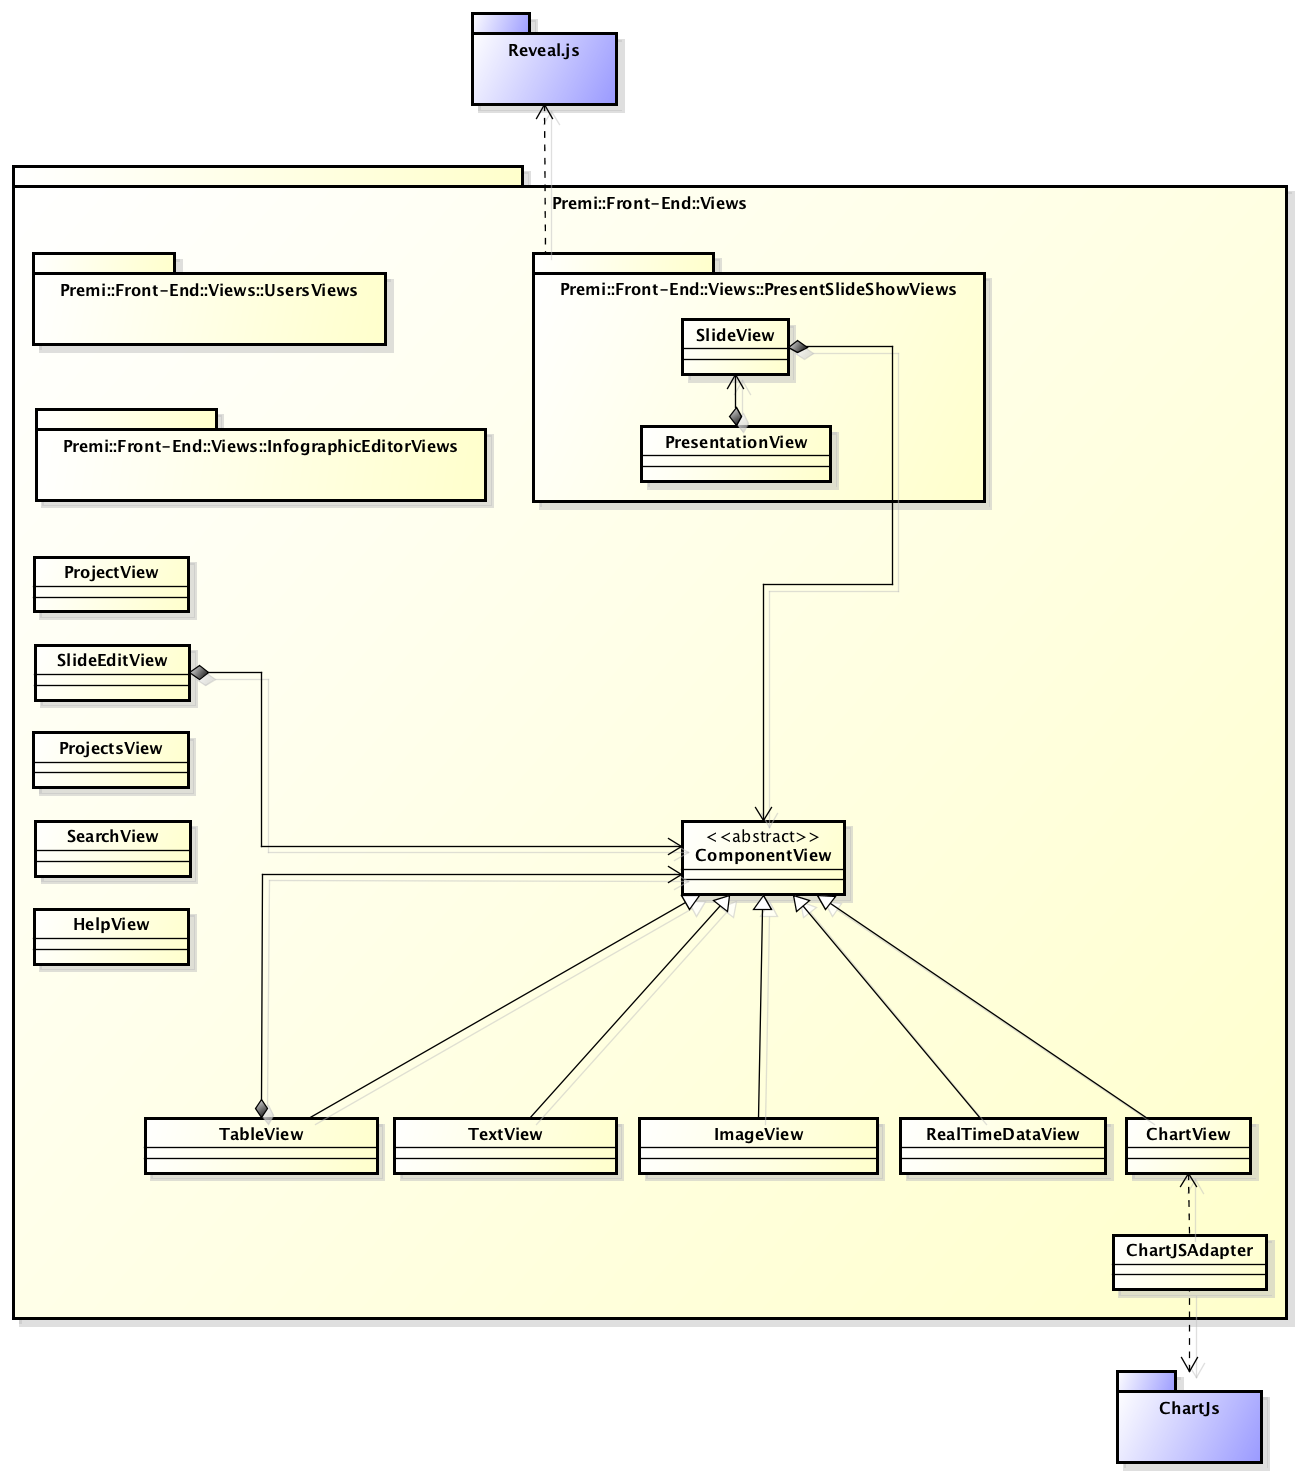
\includegraphics[width=0.7\linewidth]{img/front-end_views}
			\caption[Premi::Front-End::Views]{Premi::Front-End::Views}
		\end{figure}
		Il package contiene gli elementi per creare la parte grafica del front-end, la visualizzazione delle pagine e dell'editor del progetto.
	
	\subsubsection*{Package contenuti:}

	\begin{itemize}		
		\item Premi::Front-End::Views::UsersViews:
			\begin{itemize}
				\item \textbf{Descrizione}: classe per la gestione delle pagine riguardanti l'accesso al sito.
			\end{itemize}
		
		\item Premi::Front-End::Views::PresentSlideShowViews:
			\begin{itemize}
				\item \textbf{Descrizione}: classe per la gestione delle pagine per la visualizzazione della presentazione.
			\end{itemize}
		
		\item Premi::Front-End::Views::InfographicsEditorViews:
		\begin{itemize}
			\item \textbf{Descrizione}: classe per la gestione delle infografiche relative al progetto.
		\end{itemize}
	\end{itemize}
	
	\subsubsection*{Classi contenute:}
	\begin{itemize}
		
		\item Premi::Front-End::Views::UsersViews:
		\begin{itemize}
			\item \textbf{Descrizione}: classe per la gestione delle pagine riguardanti l'accesso al sito.
		\end{itemize}
		
		\item Premi::Front-End::Views::ProjectView:
		\begin{itemize}
			\item \textbf{Descrizione}: classe per la gestione della pagina del progetto attualmente aperto dall'utente.
		\end{itemize}
		
		\item Premi::Front-End::Views::SlideEditView:
		\begin{itemize}
			\item \textbf{Descrizione}: classe per la gestione della pagina dell'editor di una slide;
			\item \textbf{Relazioni con altre classi}:
			\begin{itemize}
				\item Premi::Front-End::Views::ComponentView.
			\end{itemize}
		\end{itemize}
		
		\item Premi::Front-End::Views::ProjectsView:
		\begin{itemize}
			\item \textbf{Descrizione}: classe per la gestione della pagina contenente i progetti creati da un utente.
		\end{itemize}
		
		\item Premi::Front-End::Views::SearchView:
		\begin{itemize}
			\item \textbf{Descrizione}: classe per la gestione della pagina per la ricerca di un progetto e la visualizzazione dei risultati.
		\end{itemize}
		
		\item Premi::Front-End::Views::HelpView:
		\begin{itemize}
			\item \textbf{Descrizione}: classe per la gestione della pagina della guida dell'applicazione.
		\end{itemize}
		
		\item Premi::Front-End::Views::ComponentView:
		\begin{itemize}
			\item \textbf{Descrizione}: classe base per la gestione grafica degli elementi che è possibile includere in una slide.
		\end{itemize}
		
		\item Premi::Front-End::Views::TableView:
		\begin{itemize}
			\item \textbf{Descrizione}: classe per la gestione grafica dell'elemento tabella che è possibile includere in una slide. Può essere composta da altri elementi della classe *::ComponentView;
			\item \textbf{Relazioni con altre classi}:
			\begin{itemize}
				\item Premi::Front-End::Views::ComponentView.
			\end{itemize}
		\end{itemize}
		
		
		\item Premi::Front-End::Views::TextView:
		\begin{itemize}
			\item \textbf{Descrizione}: classe per la gestione grafica dell'elemento casella di testo che è possibile includere in una slide;
			\item \textbf{Relazioni con altre classi}:
			\begin{itemize}
				\item Premi::Front-End::Views::ComponentView.
			\end{itemize}
		\end{itemize}
		
		\item Premi::Front-End::Views::ImageView:
		\begin{itemize}
			\item \textbf{Descrizione}: classe per la gestione grafica dell'elemento immagine che è possibile includere in una slide;
			\item \textbf{Relazioni con altre classi}:
			\begin{itemize}
				\item Premi::Front-End::Views::ComponentView.
			\end{itemize}
		\end{itemize}
		
		\item Premi::Front-End::Views::RealTimeDataView:
		\begin{itemize}
			\item \textbf{Descrizione}: classe per la gestione grafica dell'elemento di dati real-time che è possibile includere in una slide;
			\item \textbf{Relazioni con altre classi}:
			\begin{itemize}
				\item Premi::Front-End::Views::ComponentView.
			\end{itemize}
		\end{itemize}
		
		\item Premi::Front-End::Views::ChartView:
		\begin{itemize}
			\item \textbf{Descrizione}: classe per la gestione grafica dell'elemento grafico che è possibile includere in una slide;
			\item \textbf{Relazioni con altre classi}:
			\begin{itemize}
				\item Premi::Front-End::Views::ComponentView;
				\item Premi::Front-End::Views::ChartJsAdapter;
			\end{itemize}
		\end{itemize}
		
		\item Premi::Front-End::Views::ChartJsAdapter:
		\begin{itemize}
			\item \textbf{Descrizione}: classe per interfacciare l'utilizzo della classe Chart.Js con la classe ChartView;
			\item \textbf{Relazioni con altre classi}:
			\begin{itemize}
				\item Premi::Front-End::Views::ChartView;
			\end{itemize}
			\item \textbf{Relazioni con altri package}:
			\begin{itemize}
				\item Chart.Js
			\end{itemize}
		\end{itemize}
	\end{itemize}
	
	
\subsection{Premi::Front-End::Views::UsersViews}
	\subsubsection*{Informazioni sul package}
	\begin{figure}[h]
		\centering
		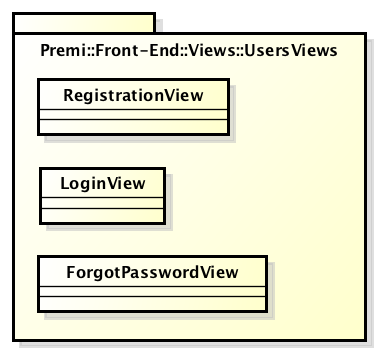
\includegraphics[width=0.7\linewidth]{img/front-end_views_usersviews}
		\caption[Premi::Front-End::Views::UsersViews]{Premi::Front-End::Views::UsersViews}
	\end{figure}
	Il package contiene le classi per creare la parte grafica dell'accesso di un utente all'applicazione.
	
	\subsubsection*{Classi contenute:}
	\begin{itemize}
		
		\item Premi::Front-End::Views::UsersViews::RegistrationView:
		\begin{itemize}
			\item \textbf{Descrizione}: classe per creare la sezione relativa alla registrazione di un nuovo utente.
		\end{itemize}
		
		\item Premi::Front-End::Views::UsersViews::LoginView:
		\begin{itemize}
			\item \textbf{Descrizione}: classe per creare la sezione relativa al login di utente già registrato.
		\end{itemize}
		
		\item Premi::Front-End::Views::UsersViews::ForgotPasswordView:
		\begin{itemize}
			\item \textbf{Descrizione}: classe per creare la sezione relativa al recupero della password per l'utente registrato.
		\end{itemize}
	\end{itemize}
	
	
\subsection{Premi::Front-End::Views::PresentSlideShowViews}
	\subsubsection*{Informazioni sul package}
	\begin{figure}[h]
		\centering
		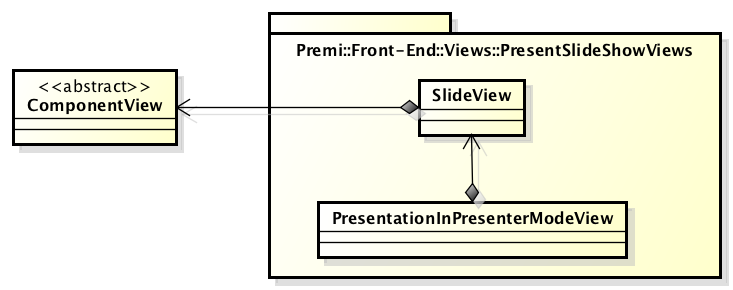
\includegraphics[width=0.7\linewidth]{img/front-end_views_presentslideshowviews}
		\caption[Premi::Front-End::Views::PresentSlideShowViews]{Premi::Front-End::Views::PresentSlideShowViews}
	\end{figure}
	Il package contiene le classi per la parte grafica relativa alla visualizzazione della presentazione da parte dell'utente.
	
	\subsubsection*{Classi contenute:}
		\begin{itemize}
			\item Premi::Front-End::Views::PresentSlideShowViews::SlideView:
			\begin{itemize}
				\item \textbf{Descrizione}: classe per creare la parte grafica di una slide nella visualizzazione di una presentazione. È composta da oggetti della classe ComponentView,o sue derivate;
				\item \textbf{Relazioni con altre classi}:
				\begin{itemize}
					\item Premi::Front-End::Views::ComponentView.
				\end{itemize}
			\end{itemize}
			
			\item Premi::Front-End::Views::PresentSlideShowViews::PresentationInPresenterModeView:
			\begin{itemize}
				\item \textbf{Descrizione}: classe per creare la parte grafica di una slide nella visualizzazione di una presentazione nella modalità presentatore. È composta da oggetti della classe SlideView in quanto la contiene implementandola;
				\item \textbf{Relazioni con altre classi}:
				\begin{itemize}
					\item Premi::Front-End::Views::PresentSlideShowViews::SlideView.
				\end{itemize}
			\end{itemize}
		\end{itemize}
		
\subsection{Premi::Front-End::Views::InfographicEditorViews}
	\subsubsection*{Informazioni sul package}
	\begin{figure}[h]
		\centering
		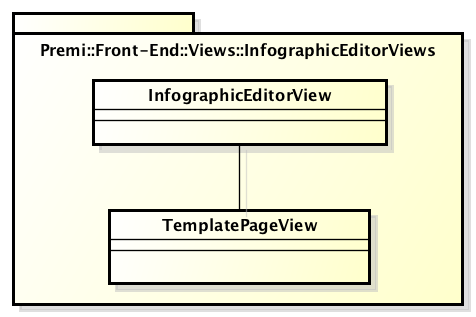
\includegraphics[width=0.7\linewidth]{img/front-end_views_infographiceditorviews}
		\caption[Premi::Front-End::Views::InfographicEditorViews]{Premi::Front-End::Views::InfographicEditorViews}
	\end{figure}
	Il package contiene le classi per la parte grafica relativa alle infografiche e alla loro creazione.

	\subsubsection*{Classi contenute:}
	\begin{itemize}
		
		\item Premi::Front-End::Views::InfographicEditorViews::InfographicEditorView:
		\begin{itemize}
			\item \textbf{Descrizione}: classe per creare un'infografica. Permette la personalizzazione di essa attraverso la selezione delle slide da usare.
		\end{itemize}
		
		\item Premi::Front-End::Views::InfographicEditorViews::TemplatePageView:
		\begin{itemize}
			\item \textbf{Descrizione}: classe che permette di creare la sezione per selezionare il template da utilizzare nell'infografica;
			\item \textbf{Relazioni con altre classi}:
			\begin{itemize}
				\item Premi::Front-End::Views::InfographicEditorViews::InfographicEditorView.
			\end{itemize}
		\end{itemize}
	\end{itemize}


\newpage

\section{Architettura Back-End}
\subsection{Back-End}
	\subsubsection*{Informazioni sul package}
		\begin{figure}[h]
			\centering
			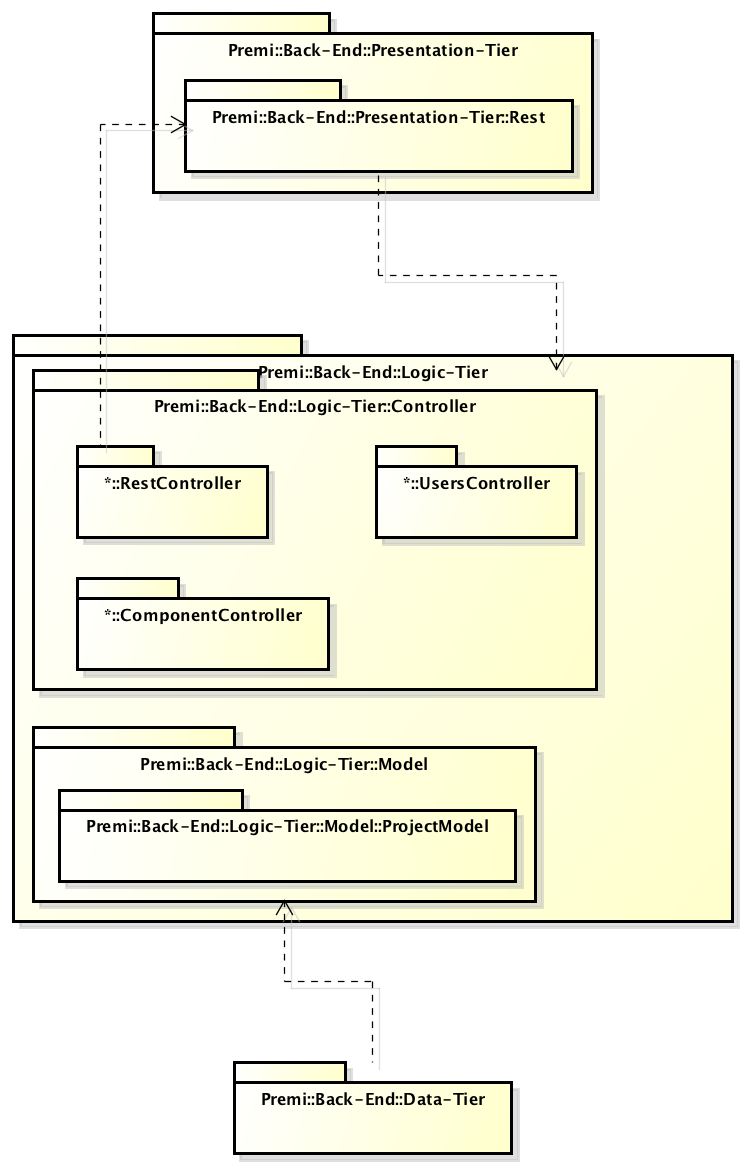
\includegraphics[width=0.9\linewidth]{img/back-end_package}
			\caption[Premi::Back-End]{Premi - Architettura di Back-End}
		\end{figure}
		Il package contiene le componenti della parte di \gls{back-end} dell'applicazione.
		
	\subsubsection*{Package contenuti}
		\begin{itemize}
			\item Premi::Presentation-Tier;
			\item Premi::Http;
			\item Premi::Model;
			\item Premi::Data-Tier.
		\end{itemize}

\newpage

\subsection{Premi::Presentation-Tier}
	\subsubsection*{Informazioni sul package}
		\begin{figure}[h]
			\centering
			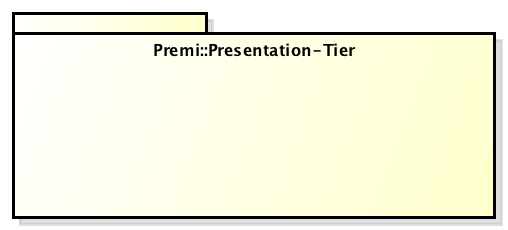
\includegraphics[width=0.5\linewidth]{img/premi_presentation-tier}
			\caption[Premi::Presentation-Tier]{Premi::Presentation-Tier}
		\end{figure}
		Il package rende possibile l'interfacciamento con il \gls{front-end}. Comunica con altri livelli attraverso i risultati di output al livello browser/client e tutti gli altri livelli della rete.
		Gestisce le chiamate \gls{REST} restituendo i risultati o eseguendo le procedure a seguito delle chiamate da parte del \gls{front-end} di uno specifico \gls{URI}. 
		
\newpage
		
\subsection{Logic Tier}
	\begin{figure}[h]
		\centering
		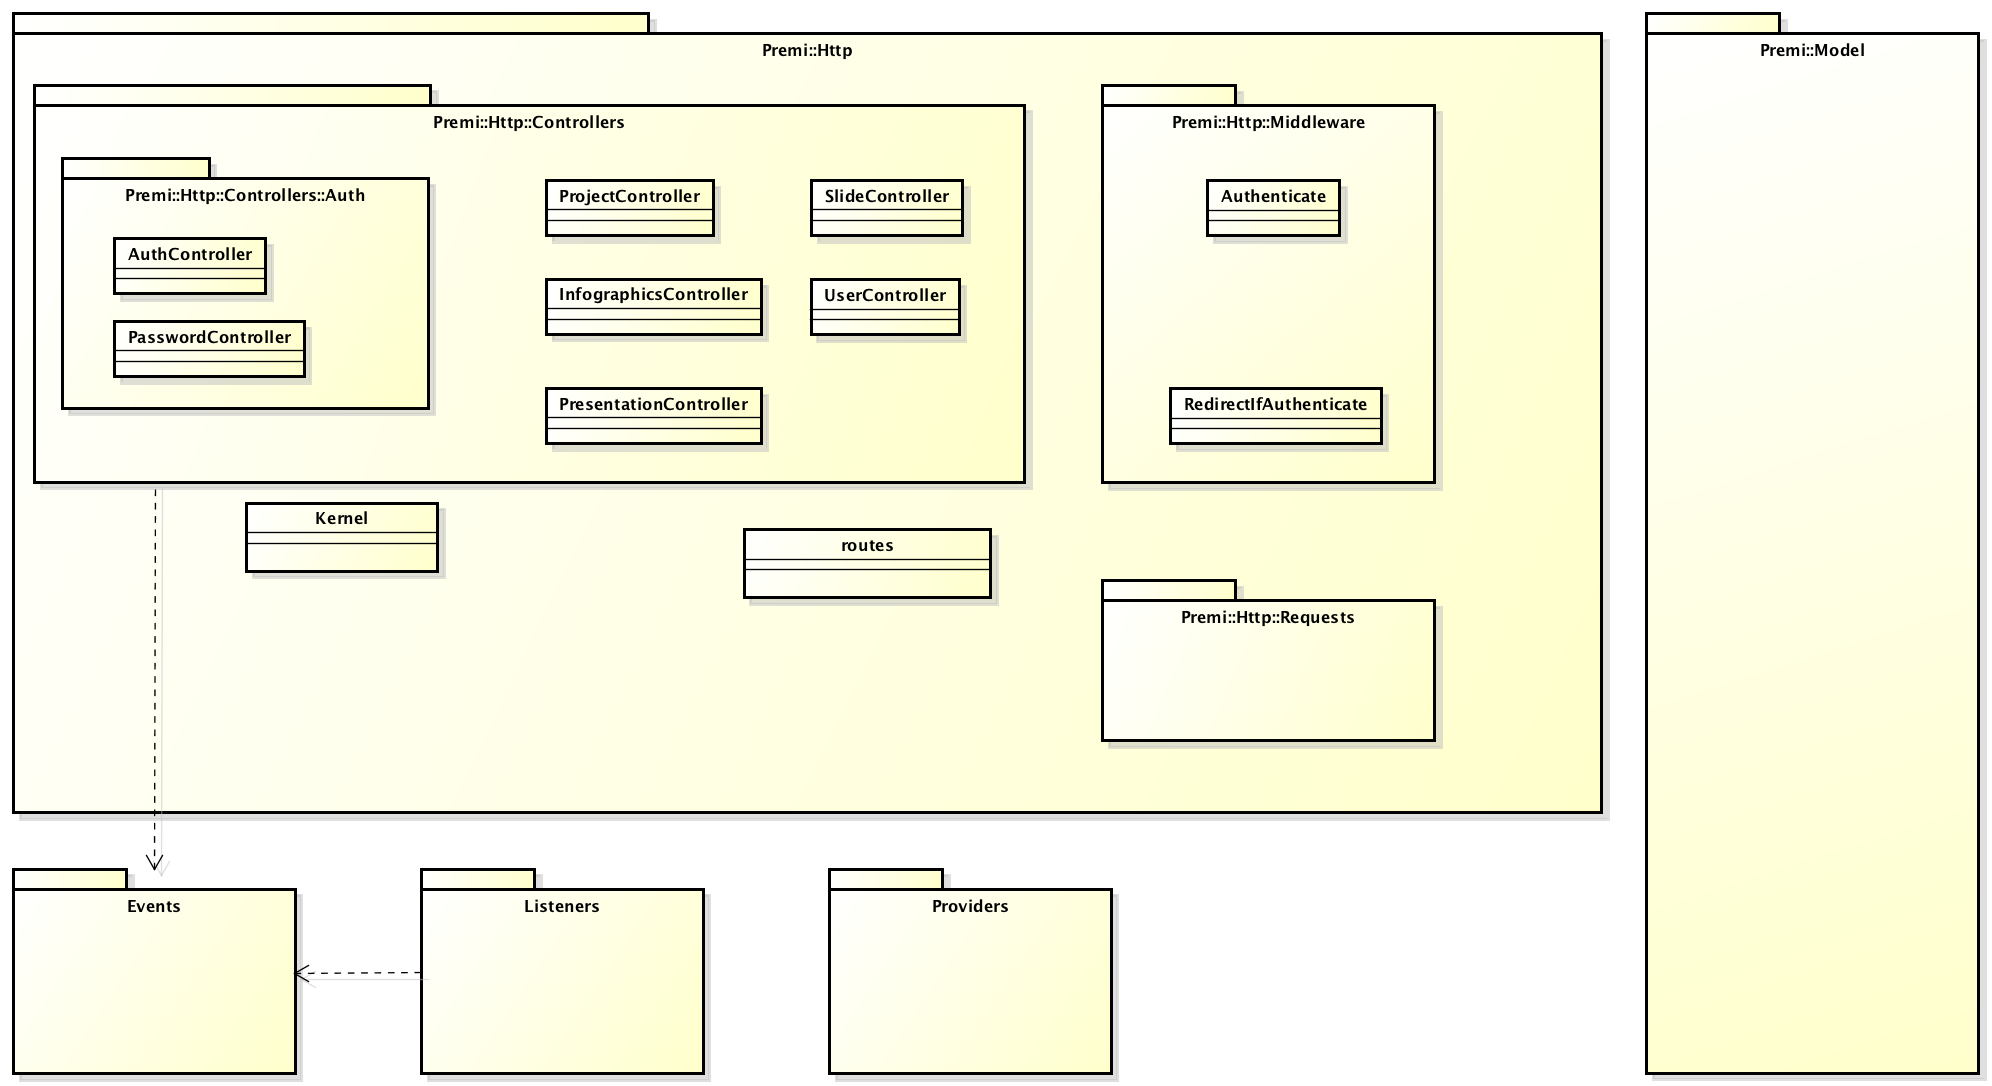
\includegraphics[width=\linewidth]{img/back-end_logic-tier_package}
		\caption[Premi::Http , Premi::Model]{Premi::Http , Premi::Model}
	\end{figure}
	Il core dell'applicazione viene implementato dal Model, che incapsulando lo stato dell'applicazione definisce i dati e le operazioni che possono essere eseguite su questi. Il package Http contiene Il componente Controller che ha la responsabilità di trasformare le interazioni dell'utente in azioni eseguite dal Model.
	
	\subsubsection*{Package contenuti}
	\begin{itemize}
		\item Premi::Http;
		\item Premi::Model.
	\end{itemize}

\newpage
\subsection{Premi::Http}
		\begin{figure}[h]
			\centering
			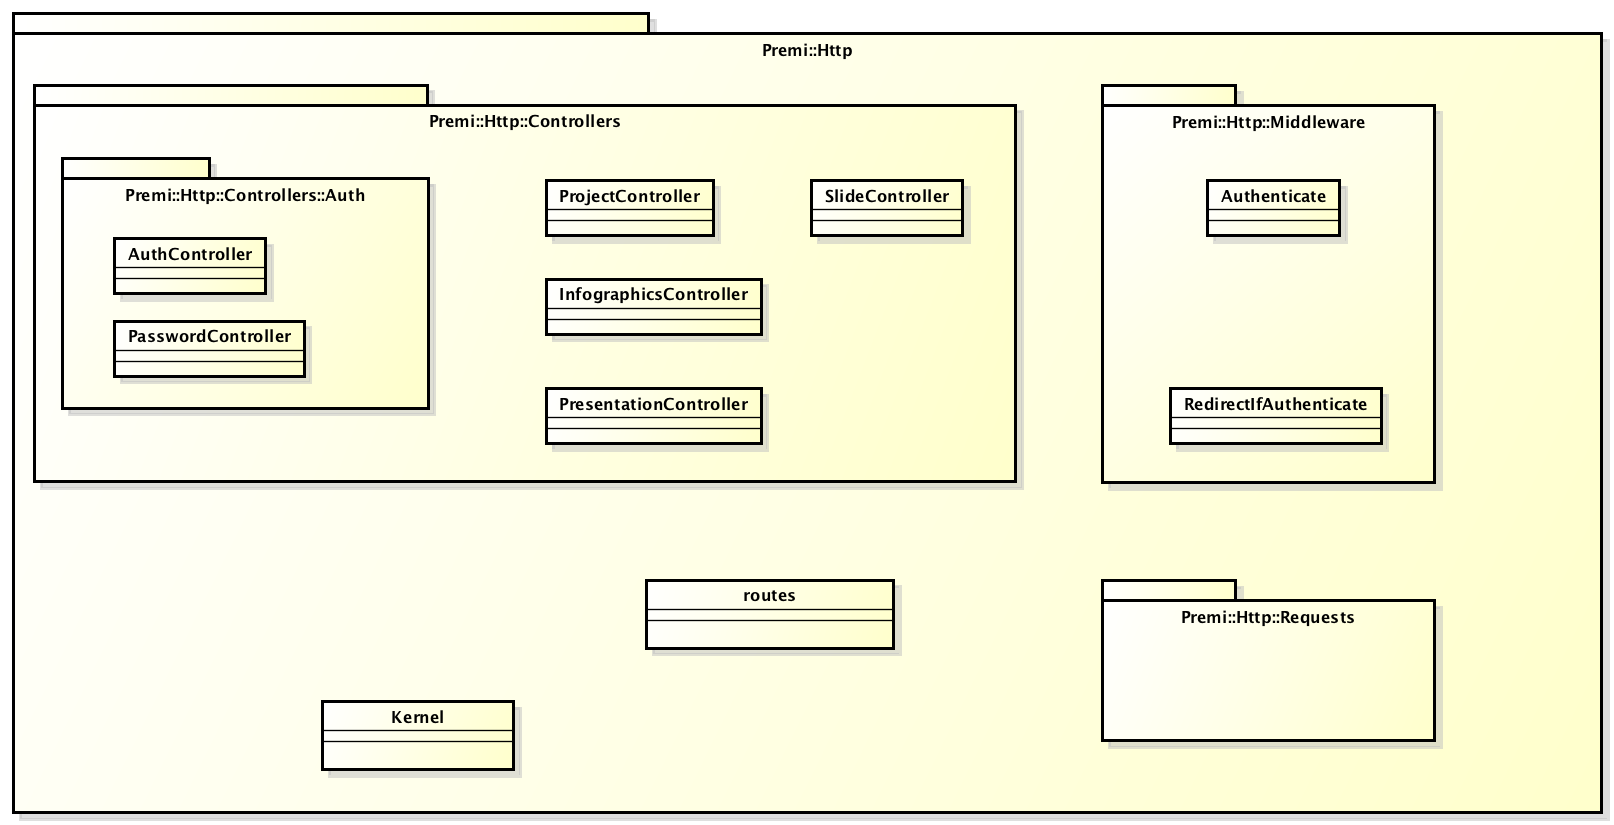
\includegraphics[width=0.9\linewidth]{img/premi_http}
			\caption[Premi::Http]{Premi::Http}
			\label{fig:premi_http}
		\end{figure}

	\subsubsection*{Informazioni sul package}
	 Il logic tier contiene a sua volta svariati package. Il package Http funziona come un'interfaccia alla vera applicazione.
	 \subsubsection*{Classi contenute}
	 \begin{itemize}
	 	\item \textbf{Routes: }collega una specifica richiesta ad un set di istruzioni ben precise;
	 	\item \textbf{Kernel: }"filtro" attraverso cui passano tutte le richieste.
	 \end{itemize}
	 \subsubsection*{Package contenuti}
		 \begin{itemize}
		 	\item Premi::Http::Controllers;
		 	\item Premi::Http::Middleware;
		 	\item Premi::Http::Requests;
		 \end{itemize}

\newpage
\subsection{Premi::Http::Controllers}
	\subsubsection*{Informazioni sul package}
	\begin{figure}[h]
		\centering
		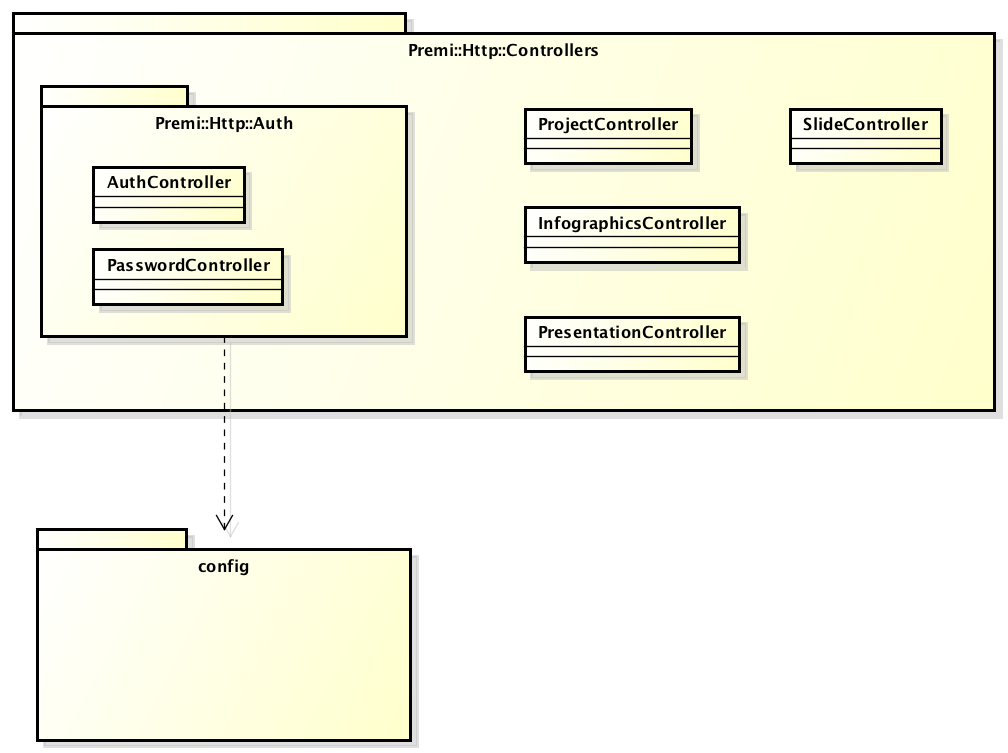
\includegraphics[width=0.9\linewidth]{img/premi_http_controllers}
		\caption[Premi::Http::Controllers]{Premi::Http::Controllers}
	\end{figure}
	Il package contiene le componenti che gestiscono la parte controller del lato \gls{back-end} dell'applicazione. 
	Sono presenti i controller per il progetto e i suoi componenti. È presente inoltre il package Auth che gestisce la parte di registrazione, autenticazione e recupero password dell'utente. 

	\subsubsection*{Package contenuti}
		\begin{itemize}
			\item Premi::Http::Controllers::Auth
		\end{itemize}
	\subsubsection*{Classi contenute}
		\begin{itemize}
			\item Premi::Http::Controllers::ProjectController;
			\item Premi::Http::Controllers::InfographicController;
			\item Premi::Http::Controllers::Presentation;
			\item Premi::Http::Controllers::SlideController.
		\end{itemize}
		
	
	\subsubsection*{Premi::Http::Controllers::Auth}
		\subsubsection*{Informazioni sul package}
		\begin{figure}[h]
			\centering
			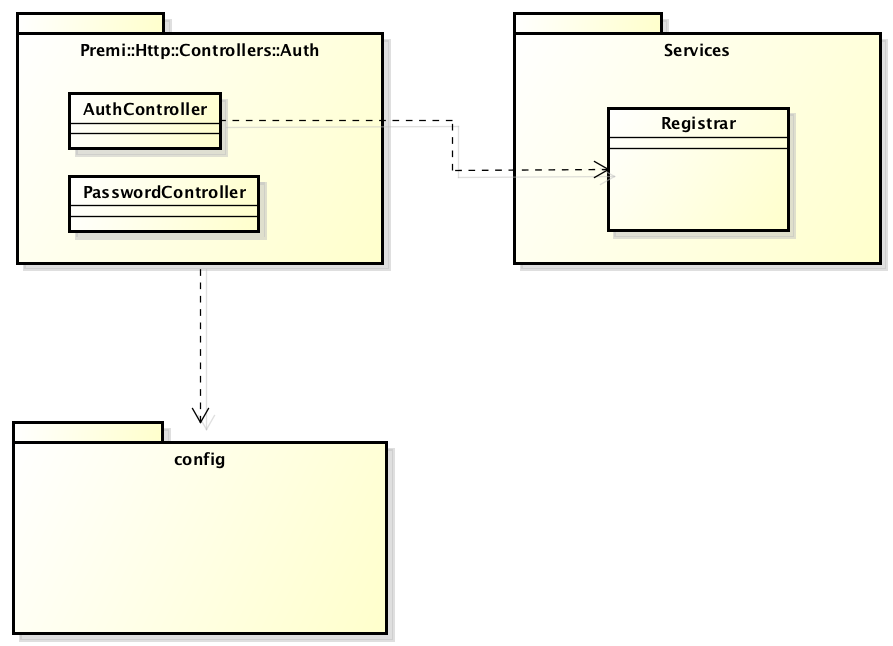
\includegraphics[width=0.9\linewidth]{img/premi_http_controllers_auth}
			\caption[Premi::Http::Controllers::Auth]{Premi::Http::Controllers::Auth}
			\label{fig:premi_http_controllers_auth}
		\end{figure}
	Laravel utilizza un semplice meccanismo di autenticazione. I file di configurazioni già documentate si trovano all'interno del package \textbf{config} che servono a ottimizzare il comportamento del servizio di autenticazione.		
	\subsubsection*{Classi contenute}
		\begin{itemize}
			\item Premi::Http::Auth::AuthController:
				\begin{itemize}
					\item \textbf{Descrizione}: AuthController gestisce le registrazioni di nuovi utenti e i loro accessi.
				\end{itemize}
			\item Premi::Http::Auth::PasswordController:
				\begin{itemize}
					\item \textbf{Descrizione:} PasswordController contiene la logica di aiuto agli utenti per la procedura di reset della password.
				\end{itemize}
		\end{itemize}
	Ognuno di questi controller usa un \gls{trait} che include i metodi necessari al loro corretto funzionamento.\\
	Per modificare i campi del form necessari alla registrazione di un nuovo utente, è sufficente modificare la classe Services::Registrar. Questa classe è responsabile della creazione e validazione dei nuovi utenti. Il metodo \textit{validator} di Registrar contiene le regole di validazione per i nuovi utenti, mentre il metodo \textit{create} di Registrar è responsabile della creazione di un nuovo record User nel database. Registrar è chiamato da AuthController tramite dei metodi contenuti nel \gls{trait} AuthenticatesAndRegistersUsers.
			
	\subsubsection*{Premi::Http::Controllers::ProjectController}
			\begin{itemize}
				\item \textbf{Descrizione}: Classe responsabile delle operazioni e della logica riguardante la gestione e la modifica di un progetto;
			\end{itemize}
			
   \subsubsection*{Premi::Http::Controllers::PresentationController}
			\begin{itemize}
				\item \textbf{Descrizione}: Classe responsabile delle operazioni e della logica riguardante la gestione e la modifica di una presentazione;
			\end{itemize}
			
	\subsubsection*{Premi::Http::Controllers::InfographicsController}
			\begin{itemize}
				\item \textbf{Descrizione}: Classe responsabile delle operazioni e della logica riguardante la gestione e la modifica di un'\gls{infografica};
			\end{itemize}
			
	\subsubsection*{Premi::Http::Controllers::SlideController}
			\begin{itemize}
				\item \textbf{Descrizione}: Classe responsabile delle operazioni e della logica riguardante la gestione e la modifica di una \gls{slide};
			\end{itemize}
		
\newpage
\subsection{Premi::Http::Middleware}
\begin{figure}[h]
\centering
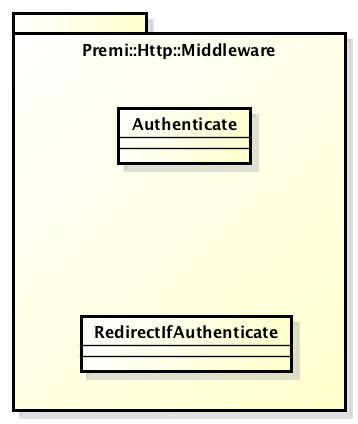
\includegraphics[width=0.7\linewidth]{img/premi_http_middleware}
\caption[Premi::Http::Middleware]{Premi::Http::Middleware}
\label{fig:premi_http_middleware}
\end{figure}

	\subsubsection*{Informazioni sul package}
	I middleware forniscono un meccanismo molto conveniente di filtraggio delle richieste HTTP in entrata.
	\subsubsection*{Classi contenute}
		\begin{itemize}
			\item \textbf{Premi::Http::Middleware::Autheticate:} verifica se l'utente dell'applicazione ha effettuato l'accesso correttamente;
			\item \textbf{Premi::Http::Middleware::RedirectIfAutheticate:} al verificarsi di un esito negativo del controllo precedente, il middleware effettua un redirect verso la schermata di login. In caso contrario, invece, tutto prosegue normalmente.
		\end{itemize}
\newpage
\subsection{Premi::Http::Request}
\begin{figure}[h]
\centering
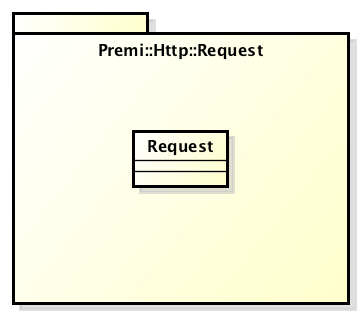
\includegraphics[width=0.7\linewidth]{img/premi_http_request}
\caption[Premi::Http::Request]{Premi::Http::Request}
\label{fig:premi_http_request}
\end{figure}
	\subsubsection*{Informazione sul package}
	La classe Facade Request garantisce l'accesso alla richiesta corrente contenuta nel container.

	
%\subsection{Premi::Back-End::Logic-Tier::Controller::ComponentController}
%	\subsubsection*{Informazioni sul package}
%		\begin{figure}[h]
%			\centering
%			\includegraphics[width=0.9\linewidth]{img/back-end_logic-tier_controller_componentcontroller}
%			\caption[Premi::Back-End::Logic-Tier::Controller::ComponentController]{Premi::Back-End::Logic-Tier::Controller::ComponentController}
%		\end{figure}
%		Il package contiene le classi dei controller per la gestione degli elementi di una \gls{slide}.
%		
%	\subsubsection*{Classi contenute}
%	\begin{itemize}
%		\item Premi::Back-End::Logic-Tier::Controller::ComponentController::ComponentController:
%		\begin{itemize}
%			\item \textbf{Descrizione}: classe che gestisce le operazioni e la logica applicativa di tutti i componenti della \gls{slide};
%			\item \textbf{Relazioni con altre classi}:
%			\begin{itemize}
%				\item Premi::Back-End::Logic-Tier::Controller::FrontController.
%			\end{itemize}
%		\end{itemize}
%		
%		\item Premi::Back-End::Logic-Tier::Controller::ComponentController::RealTimeDataController:
%		\begin{itemize}
%			\item \textbf{Descrizione}: classe che gestisce le operazioni e la logica applicativa dei componenti per i dati real-time della \gls{slide};
%			\item \textbf{Relazioni con altre classi}:
%			\begin{itemize}
%				\item Premi::Back-End::Logic-Tier::Controller::ComponentController::ComponentController.
%			\end{itemize}
%		\end{itemize}
%		
%		\item Premi::Back-End::Logic-Tier::Controller::ComponentController::ChartController:
%		\begin{itemize}
%			\item \textbf{Descrizione}: classe che gestisce le operazioni e la logica applicativa dei componenti per i grafici della \gls{slide};
%			\item \textbf{Relazioni con altre classi}:
%			\begin{itemize}
%				\item Premi::Back-End::Logic-Tier::Controller::ComponentController::ComponentController.
%			\end{itemize}
%		\end{itemize}
%		
%		\item Premi::Back-End::Logic-Tier::Controller::ComponentController::ImageController:
%		\begin{itemize}
%			\item \textbf{Descrizione}: classe che gestisce le operazioni e la logica applicativa dei componenti per le immagini della \gls{slide};
%			\item \textbf{Relazioni con altre classi}:
%			\begin{itemize}
%				\item Premi::Back-End::Logic-Tier::Controller::ComponentController::ComponentController.
%			\end{itemize}
%		\end{itemize}
%		
%		\item Premi::Back-End::Logic-Tier::Controller::ComponentController::TableController:
%		\begin{itemize}
%			\item \textbf{Descrizione}: classe che gestisce le operazioni e la logica applicativa dei componenti per le tabelle della \gls{slide};
%			\item \textbf{Relazioni con altre classi}:
%			\begin{itemize}
%				\item Premi::Back-End::Logic-Tier::Controller::ComponentController::ComponentController.
%			\end{itemize}
%		\end{itemize}
%		
%		\item Premi::Back-End::Logic-Tier::Controller::ComponentController::TextController:
%		\begin{itemize}
%			\item \textbf{Descrizione}: classe che gestisce le operazioni e la logica applicativa dei componenti per le caselle di testo della \gls{slide};
%			\item \textbf{Relazioni con altre classi}:
%			\begin{itemize}
%				\item Premi::Back-End::Logic-Tier::Controller::ComponentController::ComponentController.
%			\end{itemize}
%		\end{itemize}
%	\end{itemize}
%	

\newpage
\subsection{Premi::Model}
	\subsubsection*{Informazioni sul package}
\begin{figure}[h]
\centering
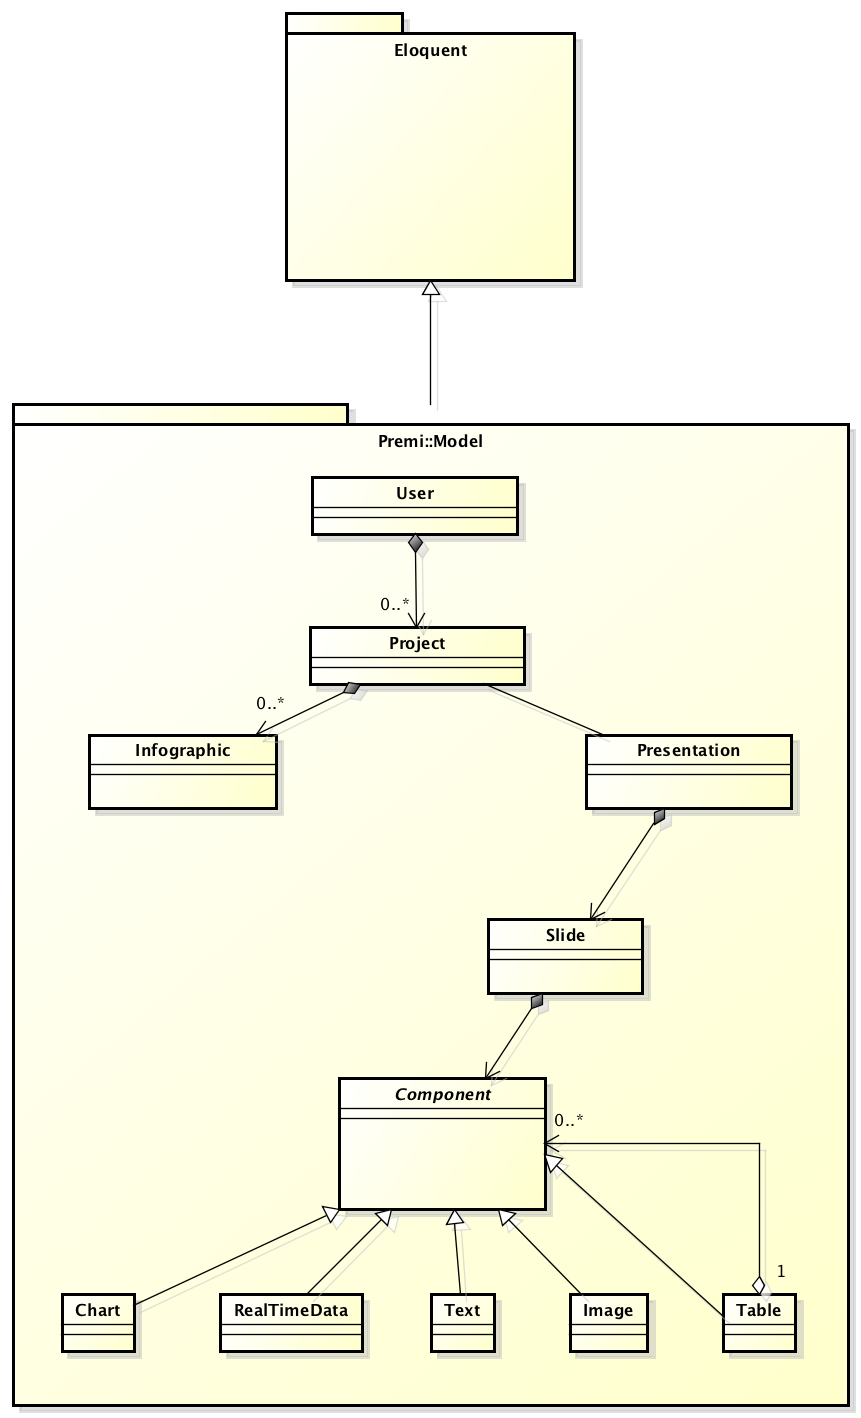
\includegraphics[width=0.7\linewidth]{img/premi_http_model}
\caption[Premi::Model]{Premi::Model}
\label{fig:premi_http_model}
\end{figure}
		Il package contiene la struttura delle classi di tutti i componenti dell'applicazione.
	
	\subsubsection*{Classi contenute}
	\begin{itemize}
		\item Premi::Model::User:
		\begin{itemize}
			\item \textbf{Descrizione:} classe contenente le informazioni di un utente.
		\end{itemize}
		\item Premi::Model::Project:
		\begin{itemize}
			\item \textbf{Descrizione}: classe base contenente le informazioni principali di un progetto.
		\end{itemize}
			
		\item Premi::Model::Infographic:
		\begin{itemize}
			\item \textbf{Descrizione:} classe che rappresenta le infografiche associate a un progetto;
			\item \textbf{Relazione con altre classi}:
			\begin{itemize}
				\item Premi::Model::Project.
			\end{itemize}
		\end{itemize}
		
		\item Premi::Model::Presentation:
		\begin{itemize}
			\item \textbf{Descrizione:} classe che rappresenta la presentazione del progetto;
			\item \textbf{Relazione con altre classi}:
			\begin{itemize}
				\item Premi::Model::Project.
			\end{itemize}
		\end{itemize}
		
		\item Premi::Model::Slide:
		\begin{itemize}
			\item \textbf{Descrizione:} classe che rappresenta le \gls{slide} che compongono una presentazione;
			\item \textbf{Relazione con altre classi}:
			\begin{itemize}
				\item Premi::Model::Project.
			\end{itemize}
		\end{itemize}
		
		\item Premi::Model::Component:
		\begin{itemize}
			\item \textbf{Descrizione:} classe base che rappresenta i componenti di cui è formata una \gls{slide};
			\item \textbf{Relazione con altre classi}:
			\begin{itemize}
				\item Premi::Model::Project.
			\end{itemize}
		\end{itemize}
		
		\item Premi::Model::Chart:
		\begin{itemize}
			\item \textbf{Descrizione:} classe che rappresenta l'elemento "grafico" che può essere inserito in una \gls{slide};
			\item \textbf{Relazione con altre classi}:
			\begin{itemize}
				\item Premi::Model::Project.
			\end{itemize}
		\end{itemize}
		
		\item Premi::Model::RealTimeData:
		\begin{itemize}
			\item \textbf{Descrizione:} classe che rappresenta l'elemento "dati real-time" che può essere inserito in una \gls{slide};
			\item \textbf{Relazione con altre classi}:
			\begin{itemize}
				\item Premi::Model::Project.
			\end{itemize}
		\end{itemize}
		
		\item Premi::Model::Text:
		\begin{itemize}
			\item \textbf{Descrizione:} classe che rappresenta l'elemento "testo" che può essere inserito in una \gls{slide};
			\item \textbf{Relazione con altre classi}:
			\begin{itemize}
				\item Premi::Model::Project.
			\end{itemize}
		\end{itemize}
		
		\item Premi::Model::Image:
		\begin{itemize}
			\item \textbf{Descrizione:} classe che rappresenta l'elemento "immagine" che può essere inserito in una \gls{slide};
			\item \textbf{Relazione con altre classi}:
			\begin{itemize}
				\item Premi::Model::Project.
			\end{itemize}
		\end{itemize}
		
		\item Premi::Model::Table:
		\begin{itemize}
			\item \textbf{Descrizione:} classe che rappresenta l'elemento "tabella" che può essere inserito in una \gls{slide};
			\item \textbf{Relazione con altre classi}:
			\begin{itemize}
				\item Premi::Model::Project.
			\end{itemize}
		\end{itemize}
	\end{itemize}
	
\subsubsection*{Informazioni su Eloquent}
Eloquent è l'ORM(Object Relational Mapping) incluso in Laravel: un'implementazione di Active Record. Tutti i model estendono  Eloquent in modo da creare e gestire l'interazione con la collection.

\subsection{Data-Tier}
\begin{figure}[h]
\centering
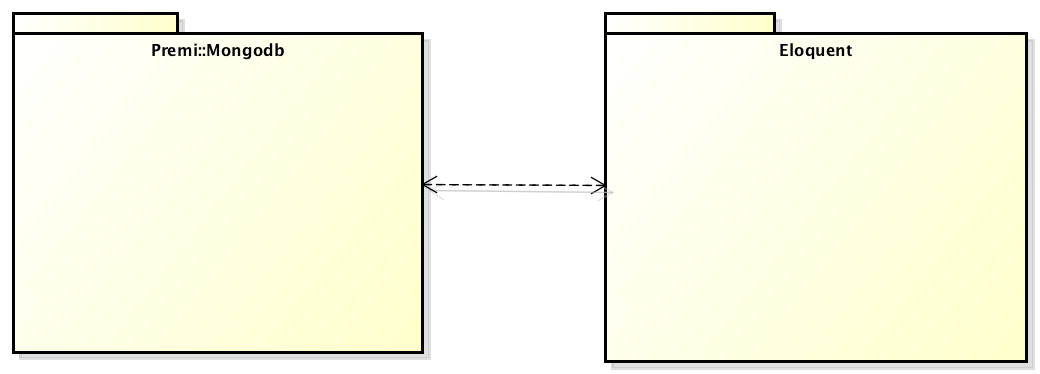
\includegraphics[width=0.7\linewidth]{img/premi_mongodb}
\caption[Premi::Mongodb]{Premi::Mongodb}
\label{fig:premi_mongodb}
\end{figure}
\subsubsection*{Informazioni sul package}
Ogni collection nel database trova una sua corrispondenza in un Model, il quale ha proprio il compito di gestire l'interazione con la collection stessa. Una volta definito il model si è pronti a selezionare un record, crearne di nuovi ed in generale lavorare con la collection. La sintassi è molto semplice: Laravel mette a disposizione le query tramite il Model Eloquent.


\newpage

%\printglossaries

\end{document}
